\begin{question}
\noindent A science laboratory uses a cylindrical container to store a chemical sample. The container is in the shape of a cylinder with radius $3.5$ cm and height $12$ cm, as shown in the diagram.

\begin{center}
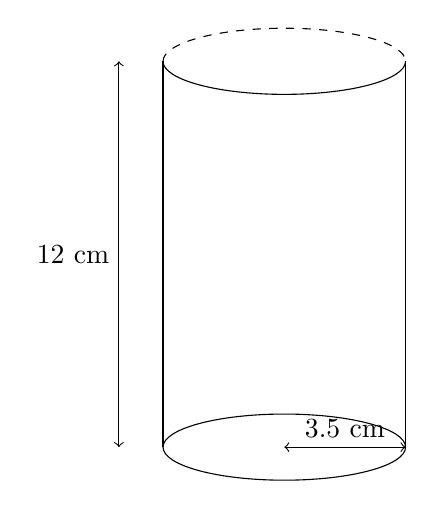
\begin{tikzpicture}[scale=0.7]
    % Draw the cylinder
    \draw (0,0) ellipse (2.2 and 0.6);
    \draw (-2.2,0) -- (-2.2,7);
    \draw (2.2,0) -- (2.2,7);
    \draw (-2.2,7) arc (180:360:2.2 and 0.6);
    \draw[dashed] (-2.2,7) arc (180:0:2.2 and 0.6);

    % Radius label
    \draw[<->] (0,0) -- (2.2,0) node[midway, above] {$3.5$ cm};

    % Height label
    \draw[<->] (-3,0) -- (-3,7) node[midway, left] {$12$ cm};
\end{tikzpicture}
\end{center}

\noindent Calculate the volume of the container.

\noindent Give your answer to 3 significant figures.
\vspace{4.5cm}
\begin{flushright}
    \answerunit{$\text{cm}^3$}{3}
\end{flushright}
\end{question}
